% !TEX encoding = UTF-8 Unicode
% -*- coding: UTF-8; -*-
% vim: set fenc=utf-8

% metodologia para cálculo do tempo: executar 4 vezes, tomar a média das 3 últimas

\chapter{Experimentos}%
\label{chap:experimentos}

Esse capítulo apresenta alguns exemplos de experimentos e de simulações computacionais com base em uma aplicação do DfAnalyzer no campo de sedimentação de dinâmica de fluidos computacionais~\cite{silva2016situ}, os quais foram executados a fim de ilustrar a implementação e a utilização do Query Preprocessor --- apresentado no \autoref{chap:rastros-de-proveniencia} ---, assim como os resultados obtidos com as consultas realizadas nos mesmos.

\section{Simulação computacional em sedimentação}

Nesse capítulo, analisamos uma aplicação do DfAnalyzer (\textit{c.f.} \autoref{sec:dfanalyzer-uma-instancia-da-arquitetura-armful}) a qual utiliza a \textit{libMesh}, uma biblioteca \textit{open-source} implementada na linguagem C++, desenvolvida para facilitar a simulação de aplicações paralelas de refinamento de malhas e elementos finitos adaptativos~\cite{boncz2008breaking}, em um resolvedor chamado \textit{libMesh-sedimentation}. O propósito dessa aplicação é simular a turbidez e perturbação de correntes de fluidos tipicamente encontradas em processos geológicos. Os sedimentos que são transportados devido à dinâmica e ao movimento dos fluidos computacionais são descritos por um modelo matemático que resulta da equação de incompressibilidade de Navier-Stokes (fluido) combinada com uma equação de transporte dominada por advecção (concentração de sedimentos). A \textit{libMesh-sedimentation} emprega um método de elementos finitos de multi-escala variacional no qual uma abordagem escalonada é utilizada para representar e simular a evolução do tempo nas equações de acoplamento entre o fluido e os sedimentos. 

Nessa aplicação os usuários empregam simulações complexas nas quais grandezas de interesse, tais como resíduos e estimativas de erros, são utilizadas para controlar de forma fina o êxito e a performance da execução~\cite{silva2016situ}. Por exemplo, a convergência ou divergência de valores de determinadas grandezas e atributos, ao longo do tempo, é uma potencial e rica fonte de informação sobre o andamento da simulação computacional. Contudo, em geral, não basta analisar uma única grandeza: frequentemente faz-se necessária a análise dos dados científicos de múltiplos arquivos, gerados em diferentes passos durante a execução do resolvedor. Nesse cenário a análise é possibilitada pelo DfAnalyzer o qual, devido a sua arquitetura em componentes herdada da ARMFUL, permite que consultas relacionadas a proveniência e aos dados científicos de múltiplos arquivos e transformações de dados sejam realizadas \textit{on-line}, ainda durante a execução da simulação computacional.

Existem duas fontes de proveniência para o componente PDG do DfAnalyzer referente a esta simulação. Uma delas é a \textit{libMesh-sedimentation solver}, mencionada anteriormente, que contribui com dados de domínio obtidos diretamente do código-fonte do resolvedor de dinâmica de fluidos computacionais. A outra é o ParaView Catalyst~\cite{ayachit2015paraview}, que é uma biblioteca com o qual o DfAnalyzer pode comunicar-se para aproveitar-se dos dados em memória gerenciados por ele e relacioná-los com o banco de dados de proveniência, além de prover recursos de visualização de regiões de interesse e de processamento de dados.

Nesse capítulo, realizamos várias consultas com um fluxo de dados \(D^{\dagger}\) baseado no resolvedor de \textbf{simulação de sedimentação de dinâmica de fluidos computacionais} mencionado nos parágrafos anteriores. Esse fluxo de dados \(D^{\dagger}\) está ilustrado na \autoref{fig:experiments-dataflow}, cujos dados foram obtidos da execução paralela desse resolvedor com 480 \textit{cores} no \textit{cluster} Lobo Carneiro\footnote{\url{http://www.nacad.ufrj.br/pt/recursos/sgiicex}} e armazenados no SGBD MonetDB.

\begin{figure}[!htb]
    \centering
    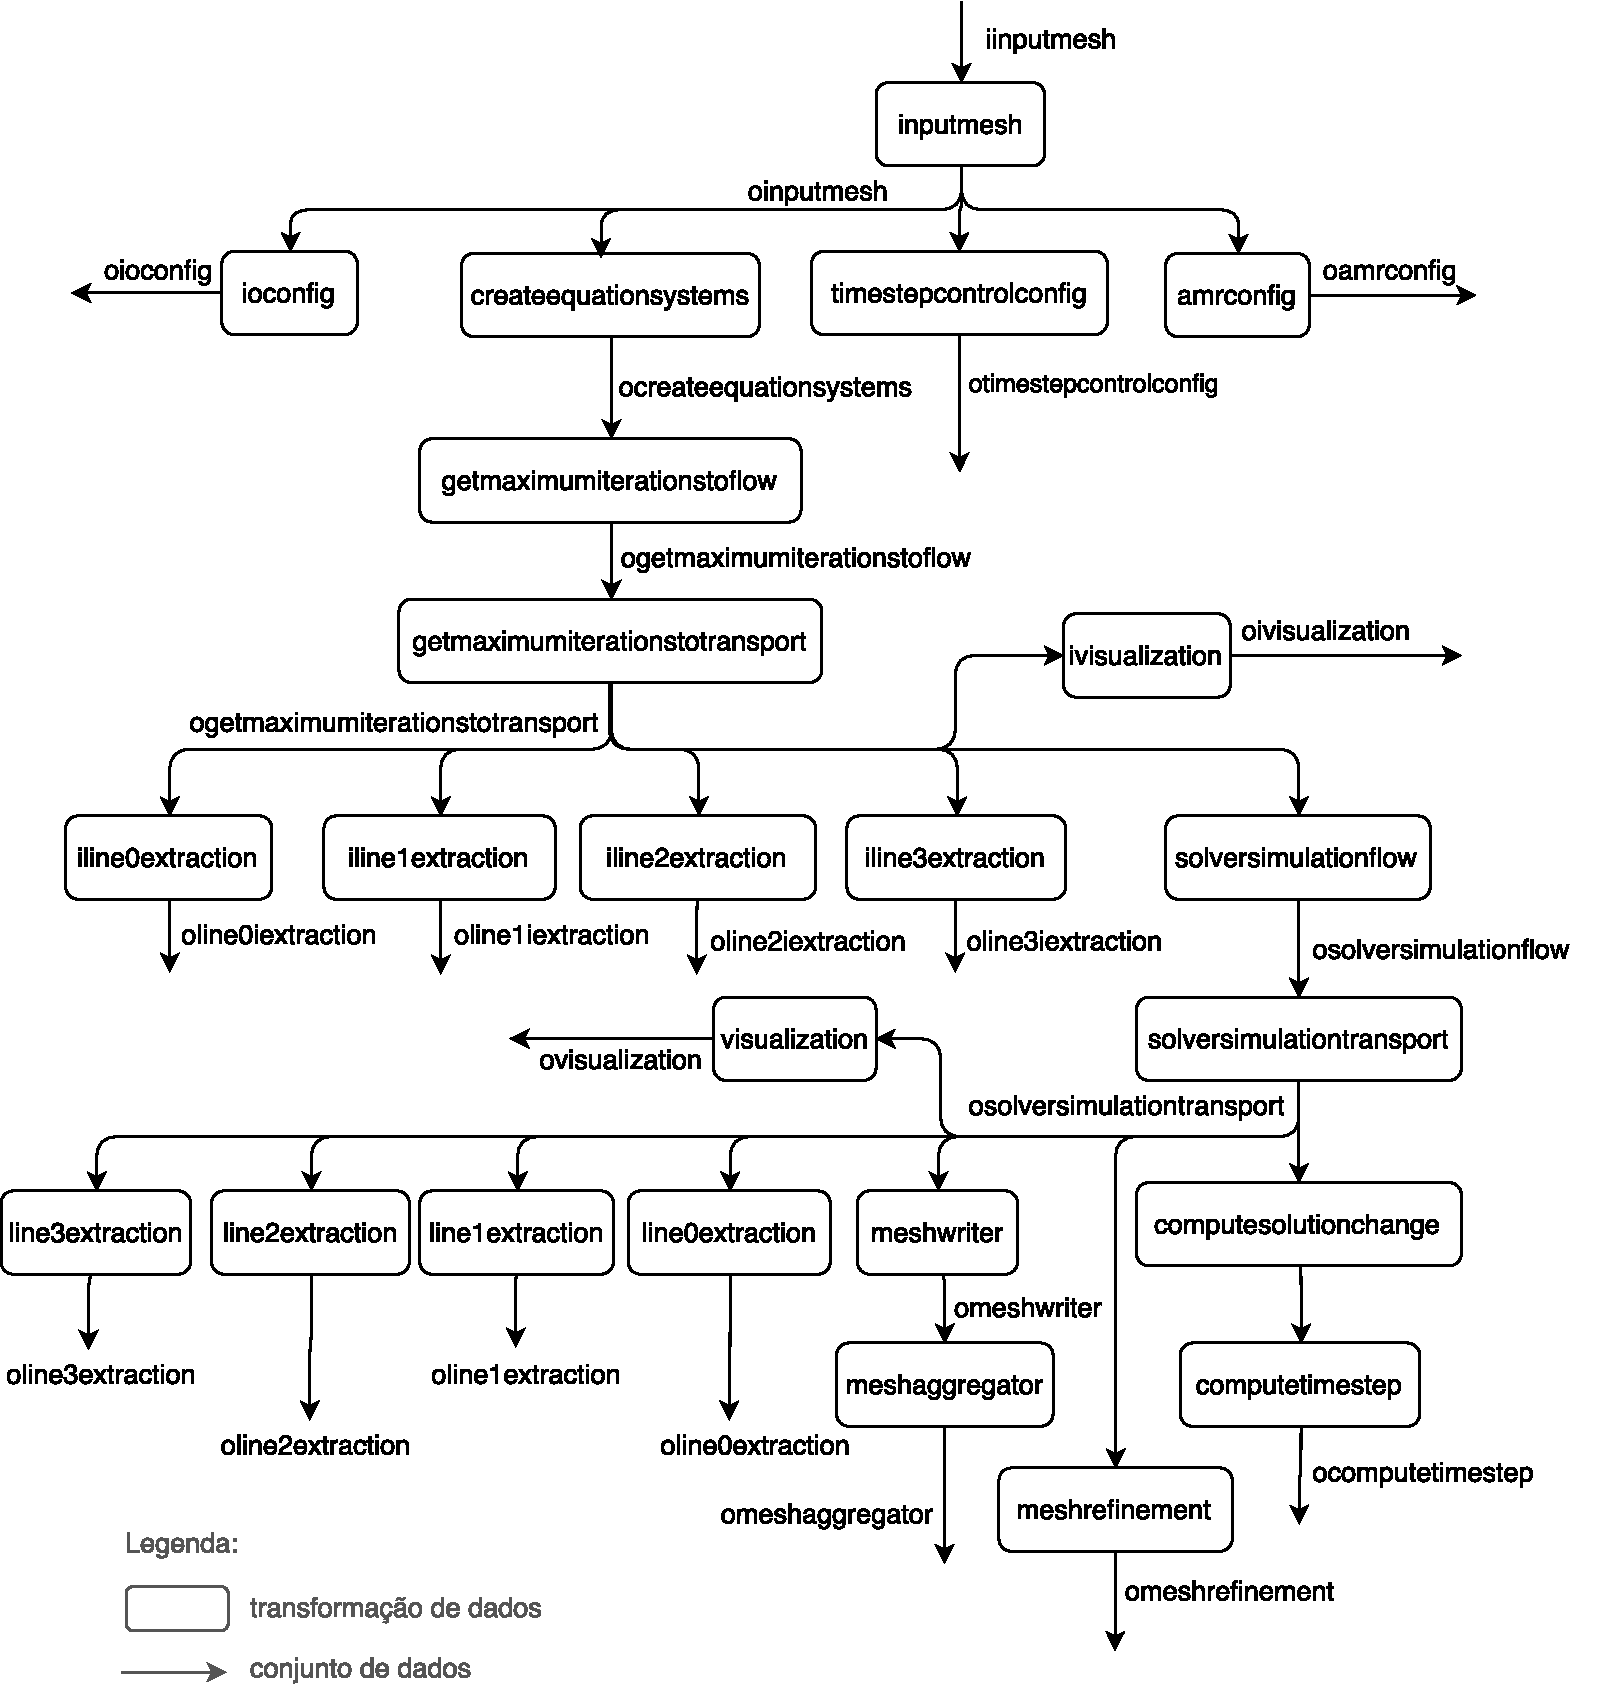
\includegraphics[width=\textwidth]{img/experiments-dataflow}
    \caption[Fluxo de dados $D^{\dagger}$ utilizado nos experimentos]{Fluxo de dados $D^{\dagger}$ utilizado nos experimentos e nas consultas do \autoref{chap:experimentos}.}%
    \label{fig:experiments-dataflow}
\end{figure}

Devido à grande quantidade de conjuntos de dados \(S^{\dagger}\) de \(D^{\dagger}\), não listamos todos os atributos de dados de \(S^{\dagger}\). No entanto, para fins de ilustração, alguns atributos de dados de \(S^{\dagger}\) podem ser visualizados na \autoref{tab:experiments-data-attributes}.

\begin{table}[htb]
    \centering
    \begin{tabular}{c|c|c|c}
\textbf{Conjunto de dados}                  & \textbf{Atributo de dados} & \textbf{Tipo}   & \makecell{\textbf{Exemplo} \\ \textbf{de Valor}}             \\ \hline
\multirow{3}{*}{osolversimulationtransport} & time                       & \makecell{ponto \\ flutuante} & $\dfrac{1}{10^5}$                                  \\ \cline{2-4}
                                            & t\_step                    & inteiro         & 0                                      \\ \cline{2-4}
                                            & meshwriter\_task\_id       & inteiro         & 17                                     \\ \hline
\multirow{2}{*}{omeshaggregator}            & xdmf                       & arquivo         & \texttt{\textasciitilde/output\_48.xmf}             \\ \cline{2-4}
                                            & n\_processors              & inteiro         & 480                                    \\ \hline
omeshrefinement                             & first\_step\_refinement    & booleano        & falso                                  \\ \hline
ovisualization                              & png                        & arquivo         & \texttt{\textasciitilde/image\_99.png} \\ \hline
oinputmesh                                  & mesh\_file                 & arquivo         & \texttt{\textasciitilde/necker3d.mesh}               \\ \hline
otimestepcontrolconfig                      & model\_name                & string          & PC11                                  
    \end{tabular}
    \caption[Exemplos de alguns atributos de dados de \(S^{\dagger}\)]{Exemplos de alguns atributos de dados de \(S^{\dagger}\).}%
    \label{tab:experiments-data-attributes}
\end{table}

% \silva{REVIEW: que tipos de arquivos ou dados são coletados na libMesh-sedimentation?. No resolvedor, capturamos dados referentes ao resíduo do solver ao resolver as equações para o fluido e os sedimentos. Para a gerência de arquivos, consideramos os raw data files nos formatos XDMF e HDF5.}

\section{Experimentos}

As consultas dos experimentos das próximas subseções, relacionadas ao Query Preprocessor, foram executadas em um computador com as seguintes especificações:

\begin{itemize}
	\item Macbook Pro Retina 2015, com o sistema operacional macOS Sierra 10.12.6;
    \item Processador Intel Core i5 2,7~GHz, com 4~CPUs;
    \item 8~GB de memória RAM do tipo DDR3.
\end{itemize}

Três consultas foram realizadas, cada uma das quais com diversos parâmetros para a função \texttt{generateSqlQuery} (\textit{c.f.} \autoref{subsec:geracao-da-consulta-em-sql}). Nota-se a distinção entre o tempo de \emph{geração} de cada consulta, referente ao tempo de processamento do QPP para gerar o código em SQL de acordo com as especificações do usuário; e o tempo de \emph{execução} de cada consulta, referente ao tempo de processamento do SGBD para retornar os resultados da consulta submetida ao mesmo.

\subsection{Consulta \#1}

% Query gerada:
%
% SELECT osolversimulationtransport.time, A% VG(oline2extraction.d)
% FROM osolversimulationtransport, oline2extraction, omeshwriter
% WHERE (osolversimulationtransport.line2extraction_task_id = oline2extraction.line2extraction_task_id)
% AND (osolversimulationtransport.meshwriter_task_id = omeshwriter.meshwriter_task_id);
% GROUP BY osolversimulationtransport.time;

% Query gerada (com GROUP BY):
%
% SELECT osolversimulationtransport.time, AVG(oline2extraction.d)
% FROM osolversimulationtransport, oline2extraction, omeshwriter
% WHERE (osolversimulationtransport.line2extraction_task_id = oline2extraction.line2extraction_task_id)
% AND (osolversimulationtransport.meshwriter_task_id = omeshwriter.meshwriter_task_id)
% GROUP BY osolversimulationtransport.time;

O objetivo da primeira consulta é a análise da média da concentração de sedimentos em uma linha extraída (\textit{i.e.}, um conjunto de pontos) de arquivos científicos, variando o tempo da simulação. Ela envolve a inspeção de três conjuntos de dados (\texttt{osolversimulationtransport}, \texttt{oline2extraction} e \texttt{omeshwriter}) de \(S^{\dagger}\) e emprega o mapeamento de atributos de dados para rastro de proveniência do tipo físico (\textit{c.f.} \autoref{subsec:rastro-de-proveniencia-do-tipo-fisico}). Apenas duas projeções são de interesse (\texttt{osolversimulation.time} e a média aritmética de \texttt{oline2extraction.d}). A especificação completa da consulta está disponível na \autoref{tab:experiments-1-especificacao}.

\begin{table}[htb]
    \centering
    \begin{tabular}{c|c}
\textbf{Argumento}          & \textbf{Valor} \\ \hline
\texttt{D}                  & $D^{\dagger}$ \\
\texttt{dsOrigins}          & \{\texttt{osolversimulationtransport}\} \\
\texttt{dsDestinations}     & \{\texttt{oline2extraction}, \texttt{omeshwriter}\} \\
\texttt{type}               & physical \\
\texttt{projections}        & \{\texttt{osolversimulationtransport.time}, \texttt{AVG(oline2extraction.d)}\} \\
\texttt{selections}         & \varnothing \\
\texttt{dsIncludes}         & \varnothing \\
\texttt{dsExcludes}         & \varnothing \\
    \end{tabular}
    \caption[Argumentos da função \texttt{generateSqlQuery} para a consulta \#1]{Especificação dos argumentos da função \texttt{generateSqlQuery} para a consulta~\#1.}%
    \label{tab:experiments-1-especificacao}
\end{table}

A consulta \#1 em SQL gerada pelo Query Preprocessor está listada no \autoref{lst:experiments-1-sql}. \textbf{Observação:} uma vez que a função de média aritmética (\texttt{AVG}) é utilizada na projeção, faz-se necessária a utilização da cláusula \texttt{GROUP BY} da linguagem SQL para que a consulta \#1 fique sintaticamente válida e bem definida. Contudo, como o Query Preprocessor não suporta essa cláusula, ela foi adicionada manualmente à consulta gerada pela função \texttt{generateSqlQuery}. O resultado da consulta \#1, executada na base de dados de \(D^{\dagger}\) carregada no MonetDB, está disponível no \autoref{lst:experiments-1-sqlresults}. Uma representação gráfica dos conjuntos de dados de \(S^{\dagger}\) utilizados nessa consulta estão realçados em vermelho na \autoref{fig:experiments-dataflow-1}.

\begin{lstlisting}[language=sql,deletendkeywords={TIME},label={lst:experiments-1-sql},caption={[Código em SQL gerado na consulta~\#1]Código em SQL gerado na consulta~\#1. Tempo médio de geração: 40,29~ms.}]
SELECT osolversimulationtransport.time, AVG(oline2extraction.d)
FROM osolversimulationtransport, oline2extraction, omeshwriter
WHERE (osolversimulationtransport.line2extraction_task_id = oline2extraction.line2extraction_task_id) 
AND (osolversimulationtransport.meshwriter_task_id = omeshwriter.meshwriter_task_id)
GROUP BY osolversimulationtransport.time;
\end{lstlisting}

\begin{center}
\begin{lstlisting}[language=sqlresults,label={lst:experiments-1-sqlresults},caption={[Resultados da consulta \#1.]Resultados da consulta \#1. Tempo médio de execução: 4,35~ms.}]
+--------------------------+--------------------------+
| time                     | AVG(oline2extraction.d)  |
+==========================+==========================+
|                1.3398483 |     1.74129306930693e-44 |
|                3.1009347 |  -1.0847045643564339e-44 |
|                5.4124618 |    7.853749801980205e-39 |
|                7.8695609 |  -1.8180726336633645e-33 |
|               10.1307669 |   1.0729463267326738e-27 |
|               12.6055519 |   1.0473414950495052e-24 |
|                       15 |   -8.768540693069305e-22 |
+--------------------------+--------------------------+
\end{lstlisting}
\end{center}

\begin{figure}[htb]
    \centering
    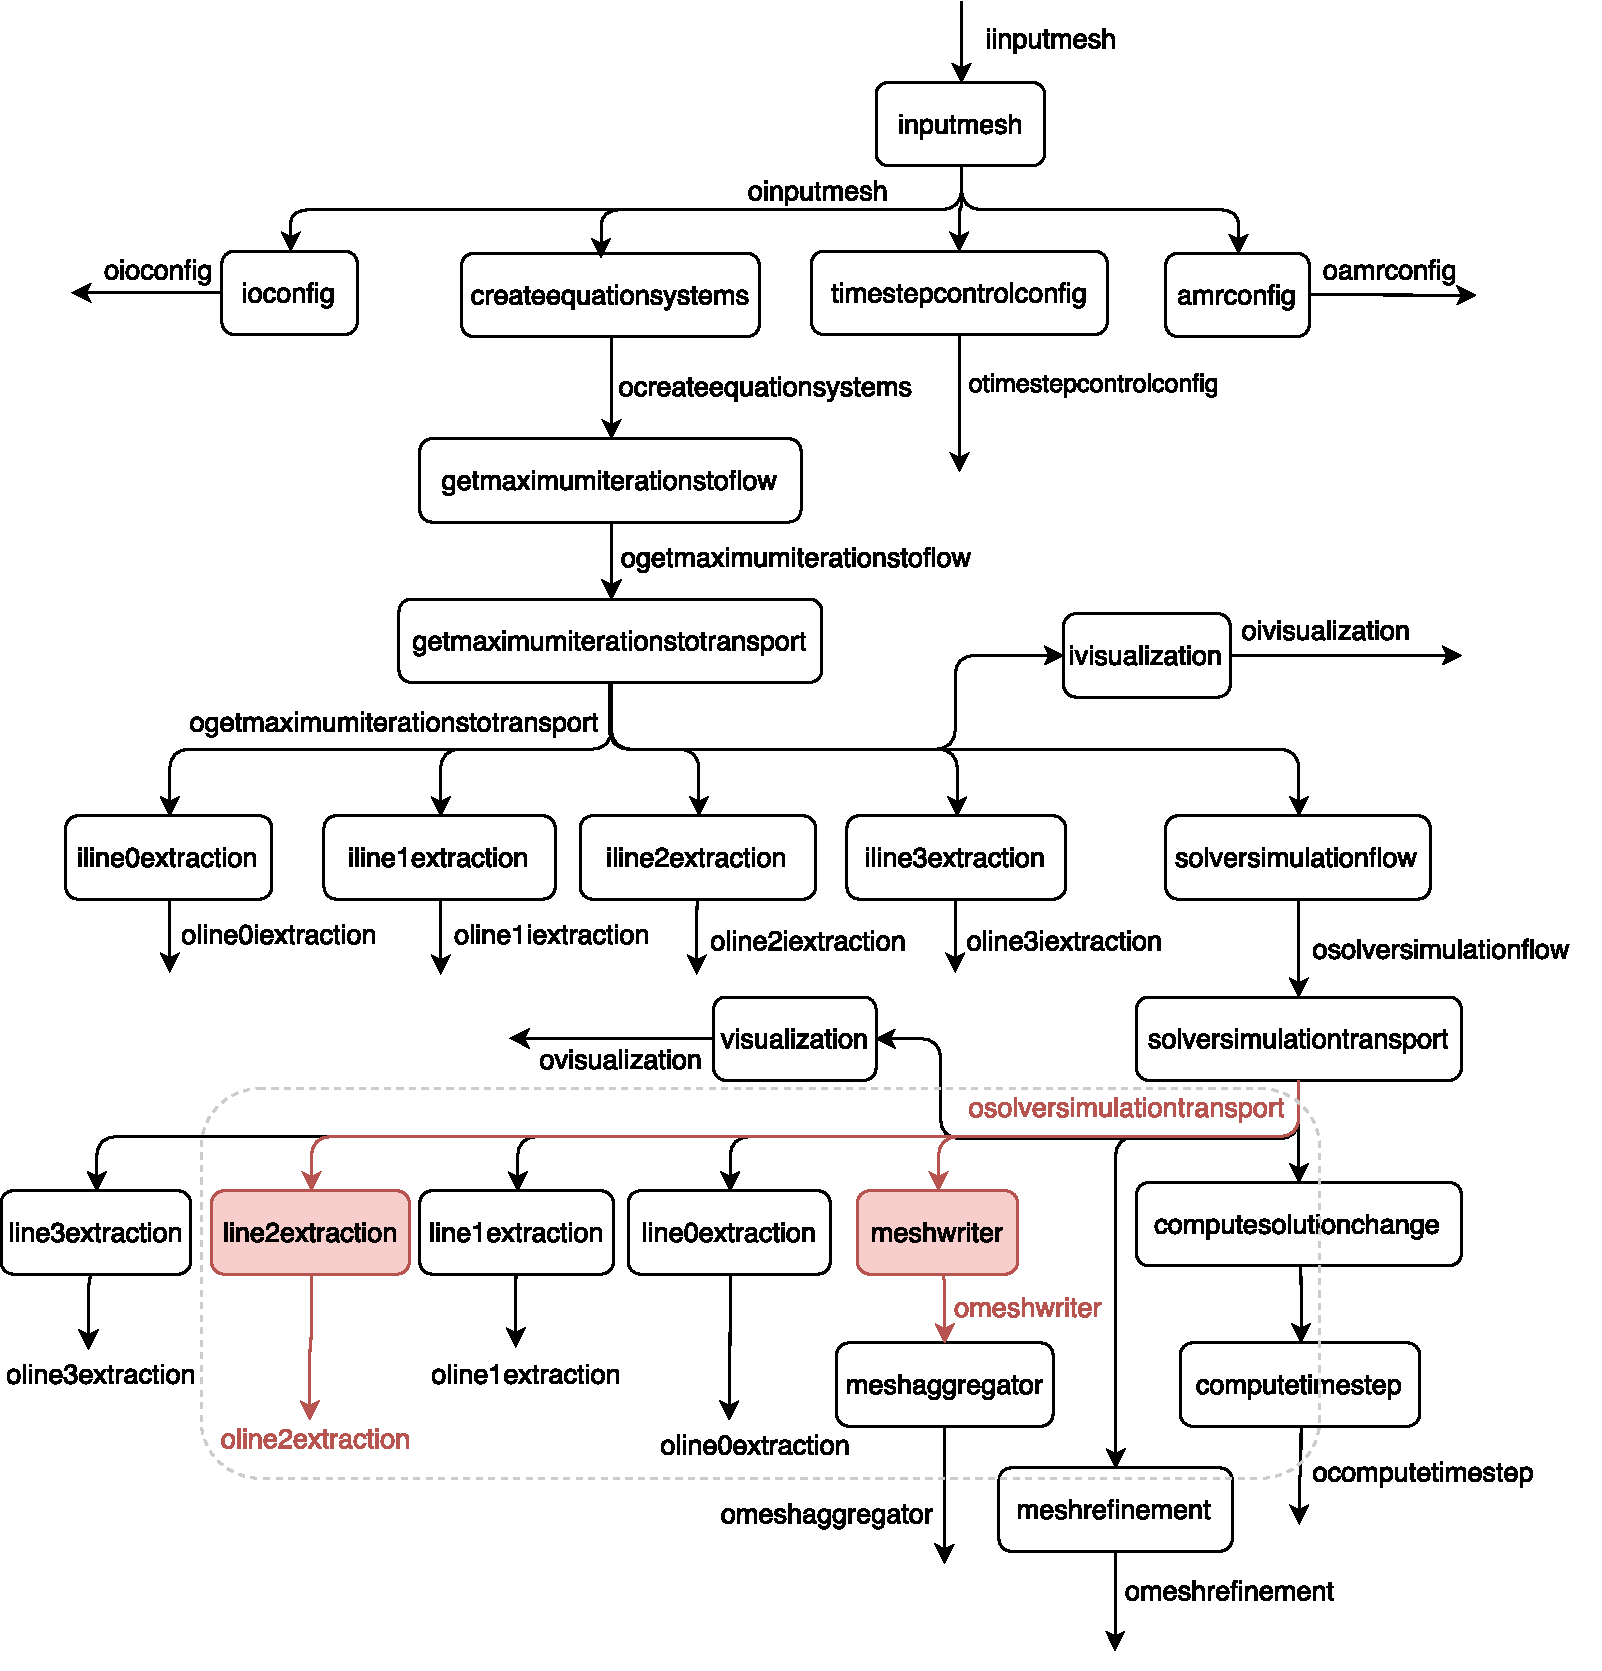
\includegraphics[width=\textwidth]{img/experiments-dataflow-1}
    \caption[Caminho do fluxo de dados \(D^{\dagger}\) rastreado na consulta \#1]{Caminho do fluxo de dados \(D^{\dagger}\) rastreado na consulta \#1.}%
    \label{fig:experiments-dataflow-1}
\end{figure}

\clearpage

\subsection{Consulta \#2}

% Query gerada:
%
% SELECT osolversimulationtransport.time, oline0extraction.points0, oline0extraction.points1, oline0extraction.points2, oline0extraction.d
% FROM osolversimulationtransport, oline0extraction, omeshwriter
% WHERE (osolversimulationtransport.time < 5.5)
% AND (oline0extraction.d > 0.1)
% AND (osolversimulationtransport.line0extraction_task_id = oline0extraction.line0extraction_task_id)
% AND (osolversimulationtransport.meshwriter_task_id = omeshwriter.meshwriter_task_id);

% Query gerada (com LIMIT):
%
% SELECT osolversimulationtransport.time, oline0extraction.points0, oline0extraction.points1, oline0extraction.points2, oline0extraction.d
% FROM osolversimulationtransport, oline0extraction, omeshwriter
% WHERE (osolversimulationtransport.time < 5.5)
% AND (oline0extraction.d > 0.1)
% AND (osolversimulationtransport.line0extraction_task_id = oline0extraction.line0extraction_task_id)
% AND (osolversimulationtransport.meshwriter_task_id = omeshwriter.meshwriter_task_id)
% LIMIT 10;

O objetivo da segunda consulta é a análise da concentração de sedimentos em uma linha extraída de arquivos de dados científicos, considerando um instante de tempo fixo e um intervalo específico de valores para a concentração de sedimentos especificada pelo usuário. Ela ilustra a inspeção de três conjuntos de dados (\texttt{osolversimulationtransport}, \texttt{oline0extraction} e \texttt{omeshwriter}) de \(S^{\dagger}\), empregando o rastro de proveniência do tipo físico. Várias projeções são de interesse para o objetivo de analisar o comportamento do conjunto de dados \texttt{oline0extraction} ao longo do tempo (segundo o atributo de dados \texttt{osolversimulationtransporte.time}). A especificação completa da consulta está disponível na \autoref{tab:experiments-2-especificacao}.

\begin{table}[htb]
    \centering
    \begin{tabular}{c|c}
\textbf{Argumento}          & \textbf{Valor} \\ \hline
\texttt{D}                  & $D^{\dagger}$ \\ \hline
\texttt{dsOrigins}          & \{\texttt{osolversimulationtransport}\} \\ \hline
\texttt{dsDestinations}     & \{\texttt{oline0extraction}, \texttt{omeshwriter}\} \\ \hline
\texttt{type}               & physical \\ \hline
\texttt{projections}        & \makecell{\{\texttt{osolversimulationtransport.time}, \\
                                          \texttt{oline0extraction.points0}, \\ 
                                          \texttt{oline0extraction.points1}, \texttt{oline0extraction.points2}, \\
                                          \texttt{oline0extraction.d}\}} \\ \hline
\texttt{selections}         & \makecell{\{\texttt{osolversimulationtransport.time < 5.5}, \\
                                          \texttt{oline0extraction.d > 0.1}\}} \\ \hline
\texttt{dsIncludes}         & \varnothing \\ \hline
\texttt{dsExcludes}         & \varnothing \\
    \end{tabular}
    \caption[Argumentos da função \texttt{generateSqlQuery} para a consulta \#2]{Especificação dos argumentos da função \texttt{generateSqlQuery} para a consulta~\#2.}%
    \label{tab:experiments-2-especificacao}
\end{table}

A consulta \#2 em SQL gerada pelo Query Preprocessor está listada no \autoref{lst:experiments-2-sql}. \textbf{Observação:} como a cláusula \texttt{LIMIT} não é implementada pelo QPP, ela foi adicionada manualmente à consulta após sua geração pela função \texttt{generateSqlQuery}. O resultado da consulta \#2, executada na base de dados de \(D^{\dagger}\) carregada no MonetDB, pode ser visualizado no \autoref{lst:experiments-2-sqlresults}. Uma representação gráfica dos conjuntos de dados de \(S^{\dagger}\) utilizados nessa consulta estão realçados em vermelho na \autoref{fig:experiments-dataflow-2}.

\begin{minipage}[c]{0.95\textwidth}
\begin{lstlisting}[language=sql,deletendkeywords={TIME},label={lst:experiments-2-sql},caption={[Código em SQL gerado na consulta~\#2]Código em SQL gerado na consulta~\#2. Tempo médio de geração: 15,45~ms.}]
SELECT osolversimulationtransport.time, oline0extraction.points0, oline0extraction.points1, oline0extraction.points2, oline0extraction.d
FROM osolversimulationtransport, oline0extraction, omeshwriter
WHERE (osolversimulationtransport.time < 5.5) 
AND (oline0extraction.d > 0.1) 
AND (osolversimulationtransport.line0extraction_task_id = oline0extraction.line0extraction_task_id) 
AND (osolversimulationtransport.meshwriter_task_id = omeshwriter.meshwriter_task_id)
LIMIT 10;
\end{lstlisting}
\end{minipage}

\begin{lstlisting}[language=sqlresults,label={lst:experiments-2-sqlresults},caption={[Resultados da consulta \#2.]Resultados da consulta \#2. Tempo médio de execução: 5,92~ms).}]
+--------------+-----------+---------+---------+----------+
| time         | points0   | points1 | points2 | d        |
+==============+===========+=========+=========+==========+
|    5.4124618 |         0 |       1 |       0 |  0.10814 |
|    5.4124618 |      0.18 |       1 |       0 |   0.1082 |
|    5.4124618 |      0.36 |       1 |       0 |  0.10825 |
|    5.4124618 |      0.54 |       1 |       0 |  0.10825 |
|    5.4124618 |      0.72 |       1 |       0 |  0.10825 |
|    5.4124618 |         0 |       1 |       0 |  0.10814 |
|    5.4124618 |      0.18 |       1 |       0 |   0.1082 |
|    5.4124618 |      0.36 |       1 |       0 |  0.10825 |
|    5.4124618 |      0.54 |       1 |       0 |  0.10825 |
|    5.4124618 |      0.72 |       1 |       0 |  0.10825 |
+--------------+-----------+---------+---------+----------+
\end{lstlisting}
% |    5.4124618 |         0 |       1 |       0 |  0.10814 |
% |    5.4124618 |      0.18 |       1 |       0 |   0.1082 |
% |    5.4124618 |      0.36 |       1 |       0 |  0.10825 |
% |    5.4124618 |      0.54 |       1 |       0 |  0.10825 |
% |    5.4124618 |      0.72 |       1 |       0 |  0.10825 |
% |    5.4124618 |         0 |       1 |       0 |  0.10814 |
% |    5.4124618 |      0.18 |       1 |       0 |   0.1082 |
% |    5.4124618 |      0.36 |       1 |       0 |  0.10825 |
% |    5.4124618 |      0.54 |       1 |       0 |  0.10825 |
% |    5.4124618 |      0.72 |       1 |       0 |  0.10825 |

\begin{figure}[htb]
    \centering
    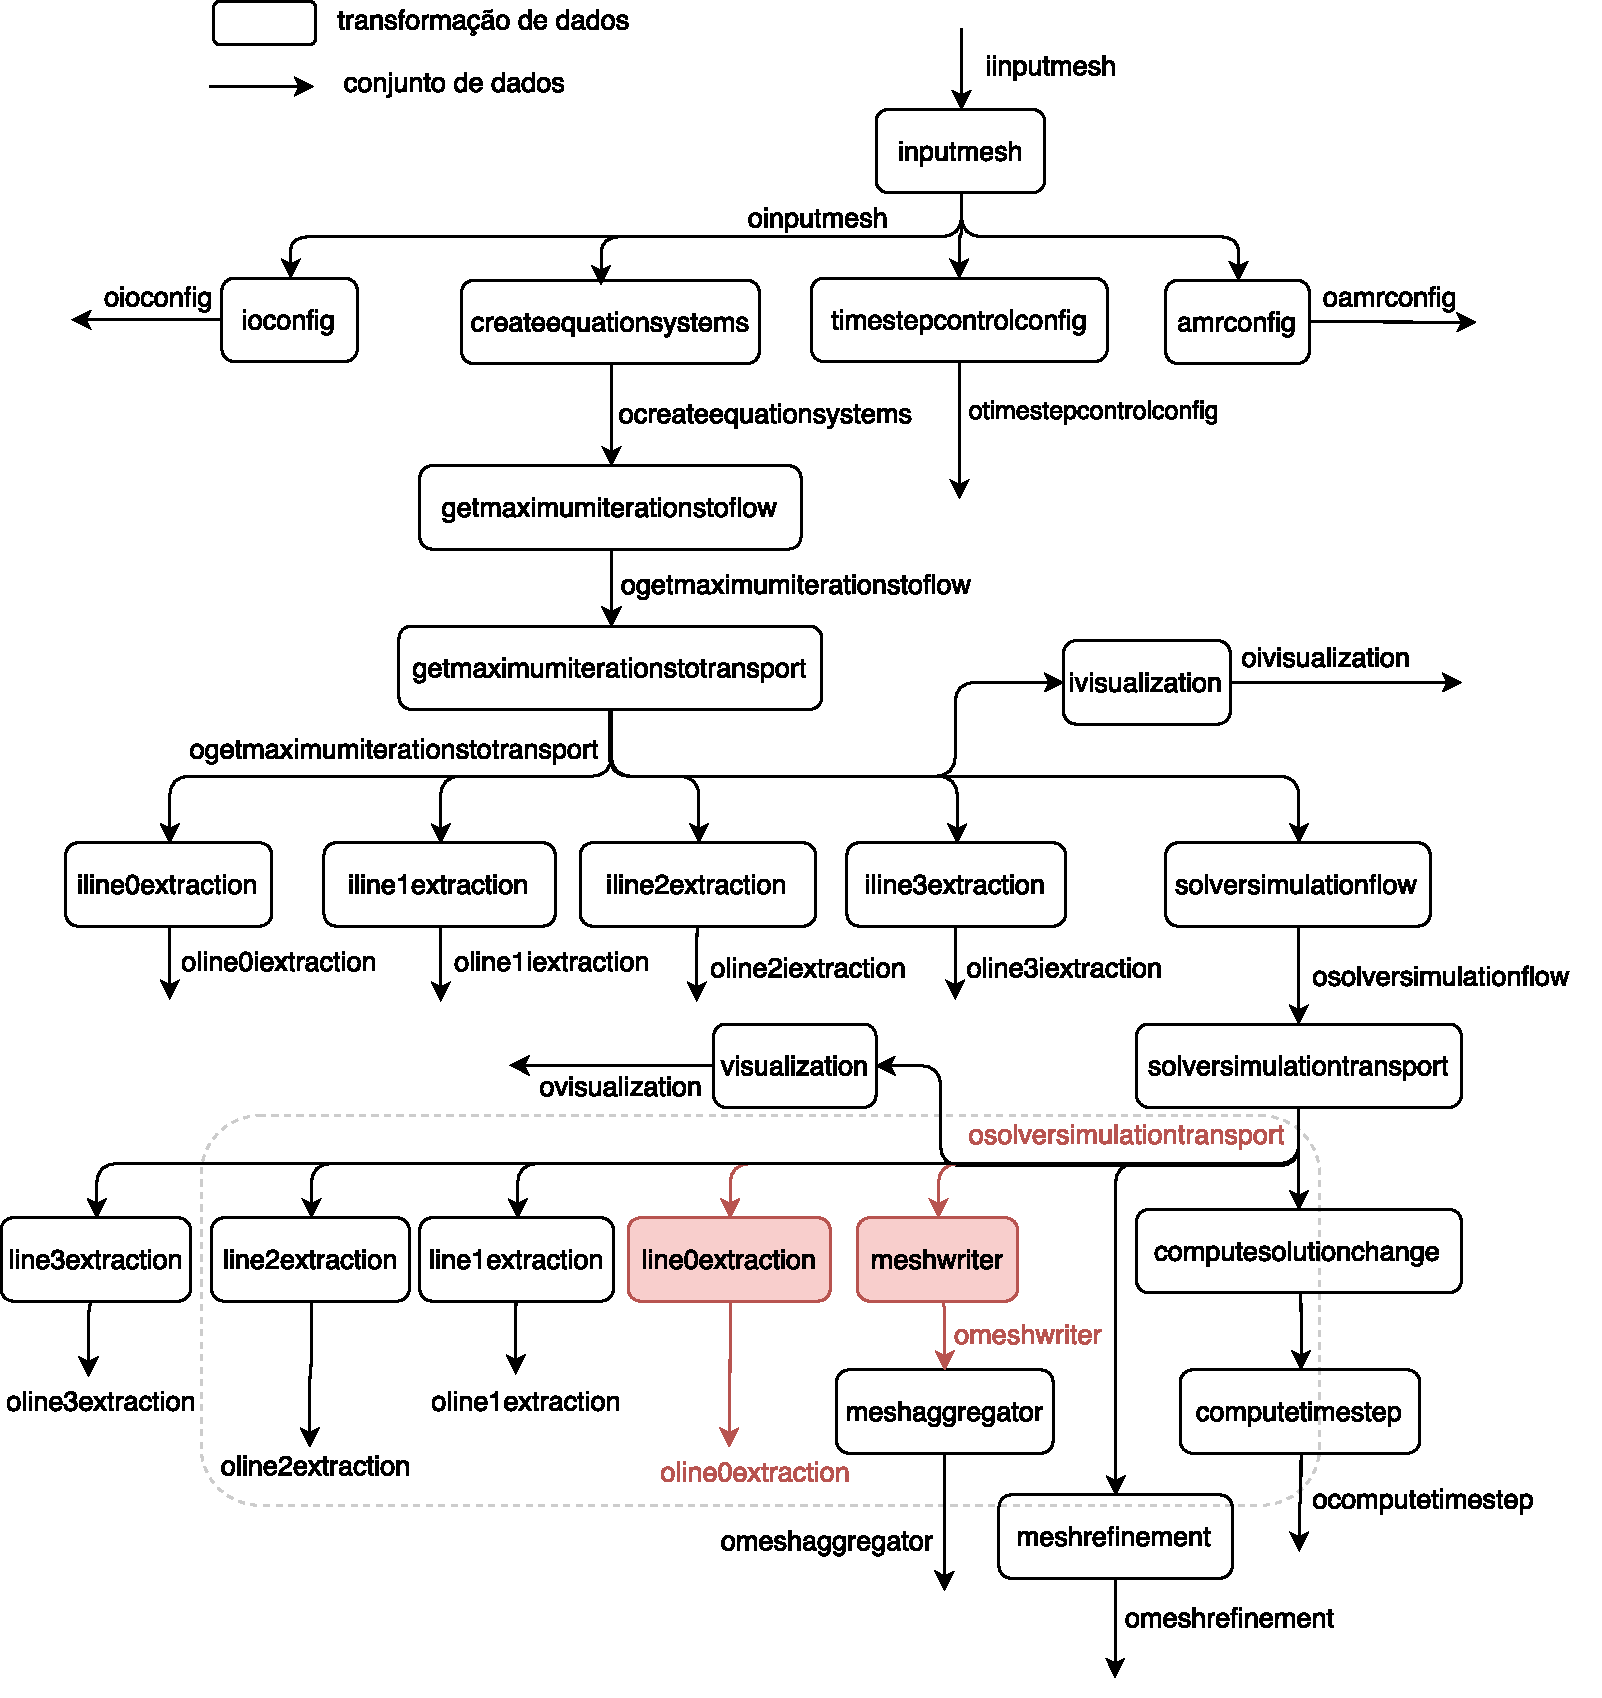
\includegraphics[width=\textwidth]{img/experiments-dataflow-2}
    \caption[Caminho do fluxo de dados \(D^{\dagger}\) rastreado na consulta \#2]{Caminho do fluxo de dados \(D^{\dagger}\) rastreado na consulta \#2.}%
    \label{fig:experiments-dataflow-2}
\end{figure}

\clearpage

\subsection{Consulta \#3}

% Query a ser gerada (antiga consulta 3):
%
% SELECT minSeds.time, minSeds.transport_n_linear_iterations,
%     minSeds.transport_final_linear_residual as minResiduals, maxSeds.transport_final_linear_residual as maxResiduals,
%     (maxSeds.transport_final_linear_residual - minSeds.transport_final_linear_residual) as variation
% FROM osolversimulationtransport as minSeds,
%     osolversimulationtransport as maxSeds,
%     (
%     SELECT seds.solversimulationtransport_task_id, seds.time, seds.transport_n_linear_iterations,
%     min(seds.transport_l) as minIter, max(seds.transport_l) as maxIter
%     FROM osolversimulationtransport as seds
%     GROUP BY seds.solversimulationtransport_task_id, seds.time, seds.transport_n_linear_iterations
%     ) as seds
% WHERE seds.time = minSeds.time
% AND seds.time = maxSeds.time
% AND minSeds.transport_l = seds.minIter
% AND maxSeds.transport_l = seds.maxIter
% AND maxSeds.transport_final_linear_residual > minSeds.transport_final_linear_residual;
%
%
% Query a ser gerada (antiga consulta 4):
%
% SELECT DISTINCT osolversimulationflow.t_step,
%        osolversimulationflow.flow_final_linear_residual,
%        osolversimulationflow.flow_norm_delta,
%        osolversimulationflow.flow_norm_delta_u,
%        osolversimulationtransport.transport_final_linear_residual,
%        osolversimulationtransport.transport_norm_delta,
%        osolversimulationtransport.transport_norm_delta_u
% FROM osolversimulationflow, osolversimulationtransport, ovisualization, omeshwriter,
% (SELECT t_step, max(r) as maxR, max(flow_l) as maxL FROM osolversimulationflow GROUP BY t_step) as fluid,
% (SELECT t_step, max(r) as maxR, max(transport_l) as maxL FROM osolversimulationtransport GROUP BY t_step) as sediments
% WHERE fluid.t_step = sediments.t_step
% AND osolversimulationflow.t_step = fluid.t_step
% AND osolversimulationflow.r = fluid.maxR
% AND osolversimulationflow.flow_l = fluid.maxL
% AND osolversimulationtransport.t_step = sediments.t_step
% AND osolversimulationtransport.r = sediments.maxR
% AND osolversimulationtransport.transport_l = sediments.maxL
% AND osolversimulationflow.solversimulationtransport_task_id = osolversimulationtransport.solversimulationtransport_task_id
% AND osolversimulationtransport.meshwriter_task_id = omeshwriter.meshwriter_task_id
% AND fluid.t_step > 20000
% LIMIT 5;

O objetivo da terceira consulta é a análise, ao longo do tempo, da evolução do resíduo linear final e da normalização de delta do fluxo e do transporte de sedimentos do \textit{solver}, assim como os arquivos de imagem (PNG) e XDMF a cada instante de tempo. A especificação completa da consulta está disponível na \autoref{tab:experiments-3-especificacao}; a fim de ilustrar a diferença entre os diversos tipos de mapeamento de atributos de dados implementados no algoritmo \autoref{lst:algorithm-attribute-mappings}, três consultas (\#3A, \#3B e \#3C) foram realizadas, cada qual com um tipo diferente no argumento \texttt{type} (\textit{physical}, \textit{logical} e \textit{hybrid}). Uma representação gráfica dos conjuntos de dados de \(S^{\dagger}\) utilizados nessas consultas estão realçados em vermelho na \autoref{fig:experiments-dataflow-3}.

\begin{table}[htb]
    \centering
    \begin{tabular}{c|c}
\textbf{Argumento}          & \textbf{Valor} \\ \hline
\texttt{D}                  & $D^{\dagger}$ \\ \hline
\texttt{dsOrigins}          & \{\texttt{osolversimulationflow}\} \\ \hline
\texttt{dsDestinations}     & \{\texttt{ovisualization}, \texttt{omeshwriter}\} \\ \hline
\texttt{type}               & physical, logical e hybrid (3 consultas distintas) \\ \hline
\texttt{projections}        & \makecell{\{%
                                          \texttt{osolversimulationflow.time}, \\
                                          \texttt{osolversimulationflow.flow\_final\_linear\_residual}, \\
                                          \texttt{osolversimulationflow.flow\_norm\_delta\_u}, \\
                                          \texttt{\tau.transport\_final\_linear\_residual}, \\
                                          \texttt{\tau.transport\_norm\_delta\_u}, \\
                                          \texttt{ovisualization.png}, \texttt{omeshwriter.xdmf}%
                                        \}} \\ \hline
\texttt{selections}         & \makecell{\{%
                                          \texttt{osolversimulationflow.time > 2}, \\
                                          \texttt{osolversimulationflow.time < 10}, \\
                                          \texttt{osolversimulationflow.r = 1}%
                                        \}} \\ \hline
\texttt{dsIncludes}         & \varnothing \\ \hline
\texttt{dsExcludes}         & \varnothing \\
    \end{tabular}
    \caption[Argumentos da função \texttt{generateSqlQuery} para as consultas \#3A, \#3B e \#3C]{Especificação dos argumentos da função \texttt{generateSqlQuery} para as consultas \#3A, \#3B e \#3C. \textbf{Observação}: \tau{} representa \texttt{osolversimulationtransport}.}%
    \label{tab:experiments-3-especificacao}
\end{table}

\begin{figure}[htb]
    \centering
    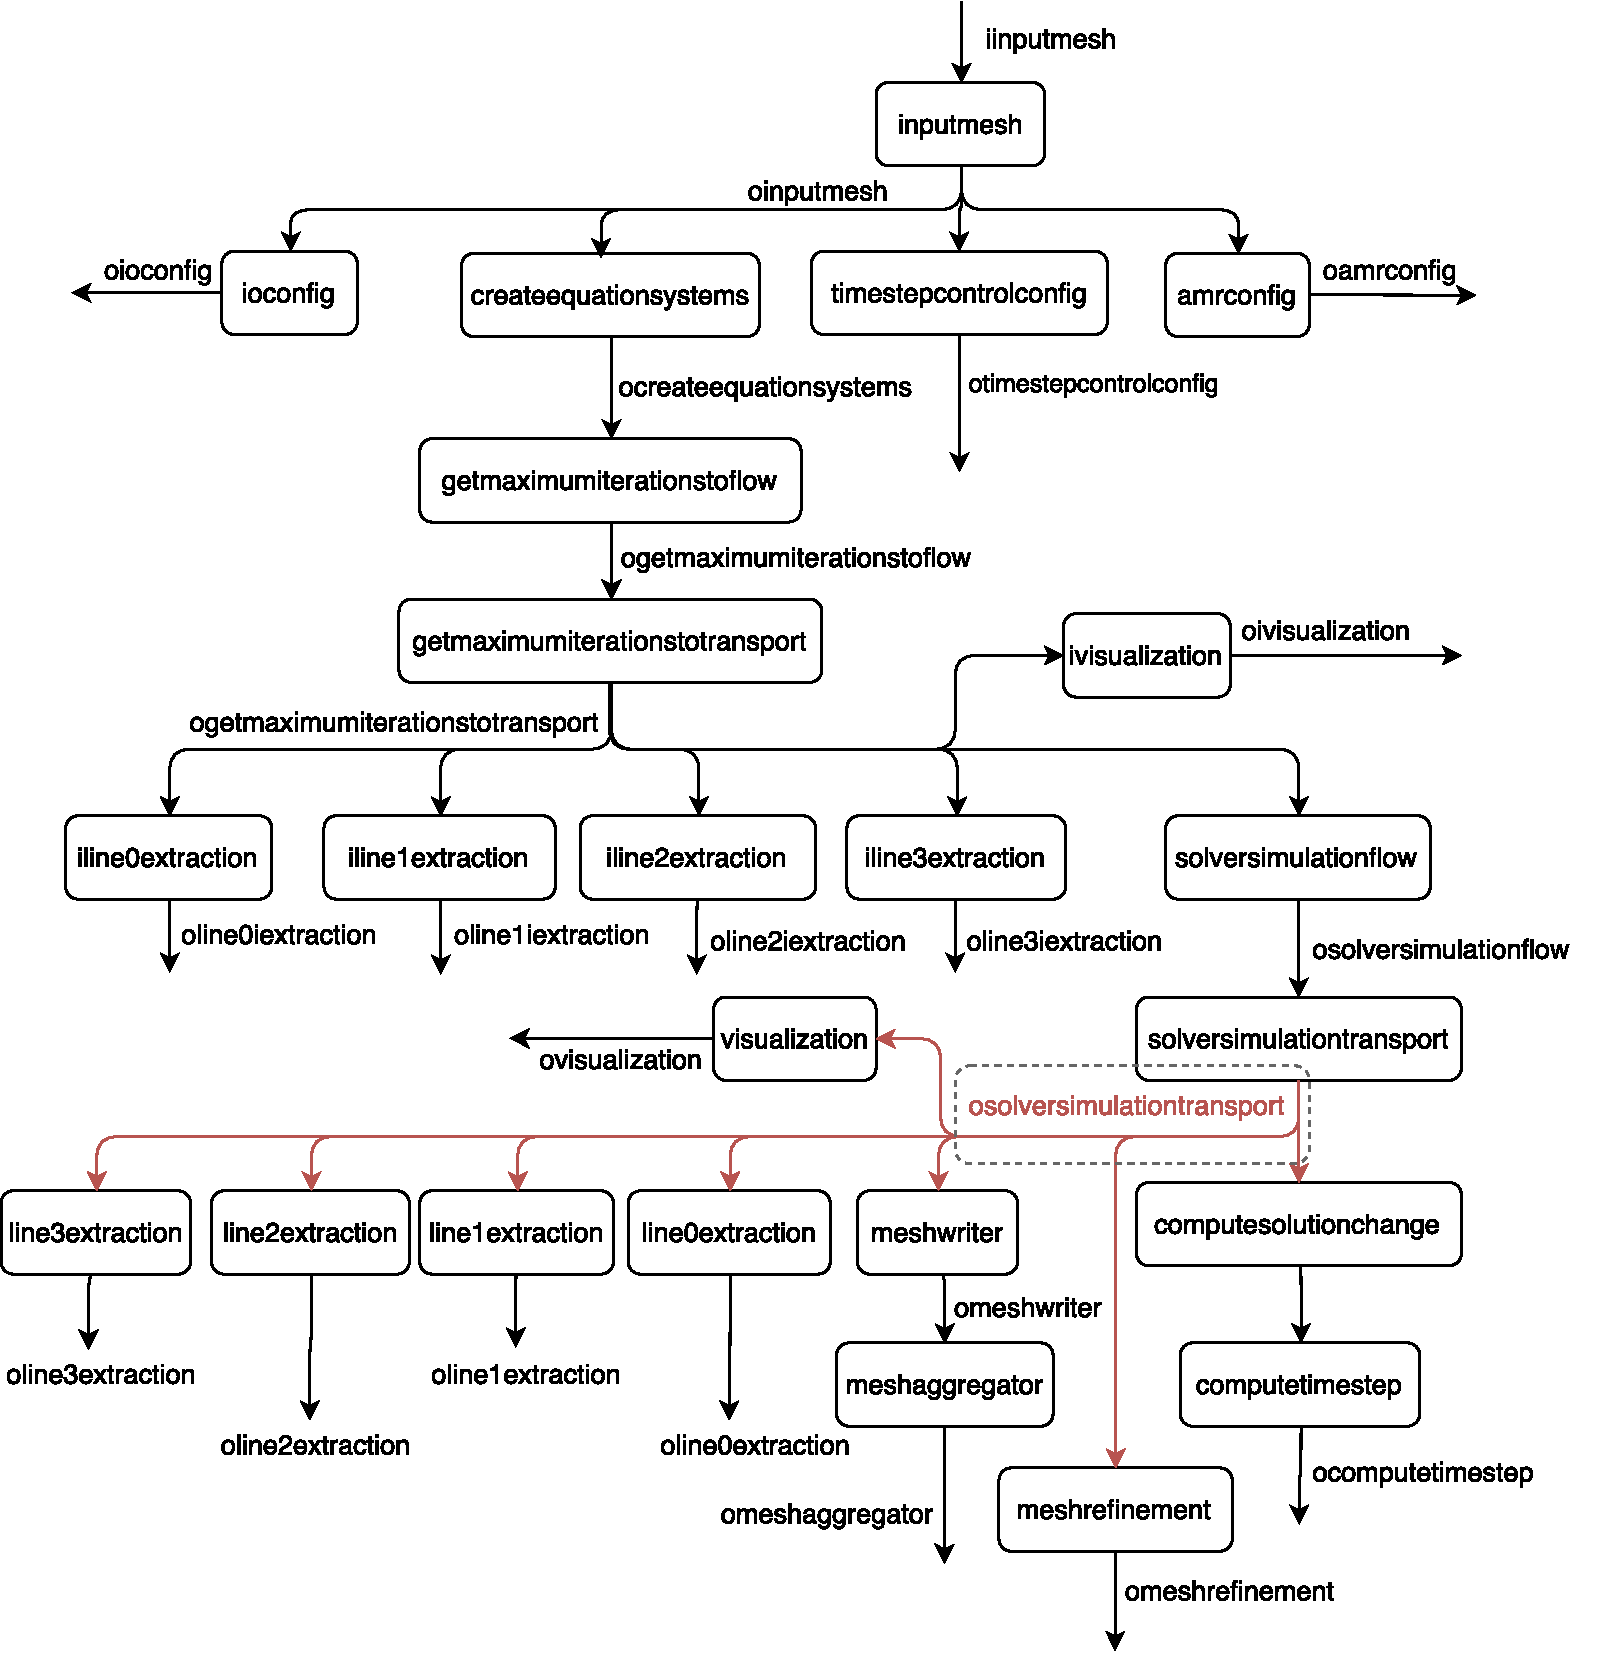
\includegraphics[width=\textwidth]{img/experiments-dataflow-3}
    \caption[Caminho do fluxo de dados \(D^{\dagger}\) rastreado nas consultas \#3A, \#3B e \#3C]{Caminho do fluxo de dados \(D^{\dagger}\) rastreado nas consultas \#3A, \#3B e \#3C.}%
    \label{fig:experiments-dataflow-3}
\end{figure}

As consultas \#3A, \#3B e \#3C, geradas em SQL pelo Query Preprocessor, estão listadas no \autoref{lst:experiments-3a-sql}, \autoref{lst:experiments-3b-sql} e \autoref{lst:experiments-3c-sql}, respectivamente. Os resultados das mesmas, executadas na base de dados de \(D^{\dagger}\) carregada no MonetDB, podem ser visualizados no \autoref{lst:experiments-3a-sqlresults}, \autoref{lst:experiments-3b-sqlresults} e \autoref{lst:experiments-3c-sqlresults}, respectivamente. Suas colunas estão na mesma ordem da especificação das projeções em \autoref{tab:experiments-3-especificacao}. Os resultados das consultas \#3A, \#3B e \#3C demonstraram, nesse exemplo, que o mapeamento lógico foi mais rico do que o físico.

\begin{lstlisting}[language=sql,deletendkeywords={TIME},deletendkeywords={TIME},label={lst:experiments-3a-sql},caption={[Código em SQL gerado na consulta~\#3A]Código em SQL gerado na consulta~\#3A. Tempo médio de geração: 31,80~ms.}]
SELECT osolversimulationflow.time, osolversimulationflow.flow_final_linear_residual, osolversimulationflow.flow_norm_delta_u, osolversimulationtransport.transport_final_linear_residual, osolversimulationtransport.transport_norm_delta_u, ovisualization.png, omeshwriter.xdmf
FROM osolversimulationflow, osolversimulationtransport, ovisualization, omeshwriter
WHERE (osolversimulationflow.time > 2) 
AND (osolversimulationflow.time < 10) 
AND (osolversimulationflow.r = 1) 
AND (osolversimulationflow.solversimulationtransport_task_id = osolversimulationtransport.solversimulationtransport_task_id) 
AND (osolversimulationtransport.visualization_task_id = ovisualization.visualization_task_id) 
AND (osolversimulationtransport.meshwriter_task_id = omeshwriter.meshwriter_task_id);
\end{lstlisting}

\begin{lstlisting}[language=sqlresults,label={lst:experiments-3a-sqlresults},caption={[Versão simplificada dos resultados da consulta \#3A.]Resultados da consulta \#3A. Tempo médio de execução: 5,11~ms.}]
+-------+-------+-------+-------+---------+---------+-----+
|3.10093|0.31609|0.00225|0.00030|. 0.00072| 9999.png|2.xmf|
|3.10093|0.31609|0.00225|0.00030|        0| 9999.png|2.xmf|
|3.10093|0.31609|0.00225|0.00025|2.224e-06| 9999.png|2.xmf|
|3.10093|0.31609|0.00225|0.00025|        0| 9999.png|2.xmf|
|5.41246|0.24713|0.00191|0.00073|0.0006674|14999.png|3.xmf|
|5.41246|0.24713|0.00191|0.00073|        0|14999.png|3.xmf|
|5.41246|0.24713|0.00191|0.00048|4.693e-06|14999.png|3.xmf|
|5.41246|0.24713|0.00191|0.00048|        0|14999.png|3.xmf|
|7.86956|0.27832|0.00563|0.00071|0.0007289|19999.png|4.xmf|
|7.86956|0.27832|0.00563|0.00071|        0|19999.png|4.xmf|
|7.86956|0.27832|0.00563|0.00026|2.551e-06|19999.png|4.xmf|
|7.86956|0.27832|0.00563|0.00026|        0|19999.png|4.xmf|
+-------+-------+-------+-------+---------+---------+-----+
\end{lstlisting}


\begin{lstlisting}[language=sql,deletendkeywords={TIME},label={lst:experiments-3b-sql},caption={[Código em SQL gerado na consulta~\#3B]Código em SQL gerado na consulta~\#3B. Tempo médio de geração: 34,36~ms.}]
SELECT osolversimulationflow.time, osolversimulationflow.flow_final_linear_residual, osolversimulationflow.flow_norm_delta_u, osolversimulationtransport.transport_final_linear_residual, osolversimulationtransport.transport_norm_delta_u, ovisualization.png, omeshwriter.xdmf
FROM osolversimulationflow, osolversimulationtransport, ovisualization, omeshwriter
WHERE (osolversimulationflow.time > 2) 
AND (osolversimulationflow.time < 10) 
AND (osolversimulationflow.r = 1) 
AND (osolversimulationflow.simulationid = osolversimulationtransport.simulationid) 
AND (osolversimulationflow.t_step = osolversimulationtransport.t_step) 
AND (osolversimulationflow.dt = osolversimulationtransport.dt) 
AND (osolversimulationflow.time = osolversimulationtransport.time) 
AND (osolversimulationflow.r = osolversimulationtransport.r) 
AND (osolversimulationtransport.simulationid = ovisualization.simulationid) 
AND (osolversimulationtransport.simulationid = omeshwriter.simulationid)
LIMIT 6; -- esse limite foi adicionado devido ao grande número de resultados dessa consulta
\end{lstlisting}

\begin{lstlisting}[language=sqlresults,label={lst:experiments-3b-sqlresults},caption={[Versão simplificada dos resultados da consulta \#3B.]Resultados da consulta \#3B. Tempo médio de execução: 19,85~ms.}]
+-------+-------+-------+-------+---------+-------+-----|
|2.00058|0.24297|0.00118|0.00034|3.404e-06|999.png|1.xmf|
|2.00058|0.24297|0.00118|0.00034|3.404e-06|999.png|2.xmf|
|2.00058|0.24297|0.00118|0.00034|3.404e-06|999.png|3.xmf|
|2.00058|0.24297|0.00118|0.00034|3.404e-06|999.png|4.xmf|
|2.00058|0.24297|0.00118|0.00034|3.404e-06|999.png|5.xmf|
|2.00058|0.24297|0.00118|0.00034|3.404e-06|999.png|6.xmf|
+-------+-------+-------+-------+---------+-------+-----+
\end{lstlisting}

\begin{lstlisting}[language=sql,deletendkeywords={TIME},label={lst:experiments-3c-sql},caption={[Código em SQL gerado na consulta~\#3C]Código em SQL gerado na consulta~\#3C. Tempo médio de geração: 43,20~ms.}]
SELECT osolversimulationflow.time, osolversimulationflow.flow_final_linear_residual, osolversimulationflow.flow_norm_delta_u, osolversimulationtransport.transport_final_linear_residual, osolversimulationtransport.transport_norm_delta_u, ovisualization.png, omeshwriter.xdmf
FROM osolversimulationflow, osolversimulationtransport, ovisualization, omeshwriter
WHERE (osolversimulationflow.time > 2) 
AND (osolversimulationflow.time < 10) 
AND (osolversimulationflow.r = 1) 
AND (osolversimulationflow.solversimulationtransport_task_id = osolversimulationtransport.solversimulationtransport_task_id) 
AND (osolversimulationflow.simulationid = osolversimulationtransport.simulationid) 
AND (osolversimulationflow.t_step = osolversimulationtransport.t_step) 
AND (osolversimulationflow.dt = osolversimulationtransport.dt) 
AND (osolversimulationflow.time = osolversimulationtransport.time) 
AND (osolversimulationflow.r = osolversimulationtransport.r) 
AND (osolversimulationtransport.visualization_task_id = ovisualization.visualization_task_id) 
AND (osolversimulationtransport.simulationid = ovisualization.simulationid) 
AND (osolversimulationtransport.meshwriter_task_id = omeshwriter.meshwriter_task_id) 
AND (osolversimulationtransport.simulationid = omeshwriter.simulationid);
\end{lstlisting}

\begin{lstlisting}[language=sqlresults,label={lst:experiments-3c-sqlresults},caption={[Versão simplificada dos resultados da consulta \#3C.]Resultados da consulta \#3C. Tempo médio de execução: 11,88~ms.}]
+-------+-------+-------+-------+---------+---------+-----+
|3.10093|0.31609|0.00225|0.00025|2.224e-06| 9999.png|2.xmf|
|3.10093|0.31609|0.00225|0.00025|        0| 9999.png|2.xmf|
|5.41246|0.24713|0.00191|0.00048|4.693e-06|14999.png|3.xmf|
|5.41246|0.24713|0.00191|0.00048|        0|14999.png|3.xmf|
|7.86956|0.27832|0.00563|0.00026|2.551e-06|19999.png|4.xmf|
|7.86956|0.27832|0.00563|0.00026|        0|19999.png|4.xmf|
+-------+-------+-------+-------+---------+---------+-----+
\end{lstlisting}
